\chapter{Experiments and Results}\label{chapter:measurements}

This chapter delves into the empirical exploration conducted to understand the interplay between various control variables and the performance of Matrix Profiling algorithms on the Cerebras Wafer Scale Engine (WSE).

In this chapter, we systematically investigate the influence of four pivotal control variables: \texttt{Time Series}, \texttt{Tile Size}, \texttt{Window Size}, and \texttt{Resource Rectangle}, on the performance and accuracy of Matrix Profiling computations on the Cerebras WSE. By meticulously varying these parameters and analyzing their impact on computational metrics such as execution time, memory utilization, and result fidelity, we aim to unravel insights crucial for optimizing Matrix Profiling workflows on this cutting-edge hardware platform.

We also outline our experimental methodology, detailing the setup, execution, and analysis of Matrix Profiling experiments on the Cerebras WSE. Through rigorous empirical investigation, we endeavor to shed light on the intricate relationship between control variables and Matrix Profiling performance, ultimately contributing to the advancement of time series analysis techniques on state-of-the-art computing architectures.

Our findings hold implications for researchers and practitioners seeking to harness the potential of novel hardware platforms like the Cerebras WSE for accelerating Matrix Profiling tasks. By elucidating the optimal configurations and parameters for Matrix Profiling experiments, we aim to facilitate the development of scalable, high-performance solutions tailored to the demands of modern data analysis workflows.

\clearpage

\section{Experimentation Model} \label{section:model}

In this chapter, we delve into a series of experiments aimed at elucidating the impact of various control variables on the performance of Matrix Profiling algorithms executed on the Cerebras Wafer Scale Engine (WSE), The implementation targeted the \texttt{Cerebras SDK 1.0.0}. These experiments are guided by the following control variables:

\begin{itemize}
    \item \textbf{Time Series (\textit{s})}: The length of the time series data being analyzed.
    \item \textbf{Tile Size (\textit{$t_s$})}: The size of the tile allocated to a single PE, which directly influences the parallelism and performance.
    \item \textbf{Window Size (\textit{m})}: The size of the sliding window used for local pattern discovery within the time series data. It is fixed to $6$ for all the experiments unless specified.
    \item \textbf{Resource Rectangle (\textit{r\_r})}: The configuration of resources allocated within the Cerebras WSE for executing the Matrix Profiling algorithm. It consists of 2 variables, width $w$, height $h$.
\end{itemize}

These control variables serve as the foundation for our experimental design, allowing us to systematically explore their implications on the overall execution and performance of the Matrix Profiling algorithm on the Cerebras WSE-2. The time series used for the experiments are random walk time series generated uniquely for each test case.

The Matrix Profiling algorithm exhibits a time complexity of \(O(s^2)\), where \(s\) represents the length of the time series data. The time complexity of the tiled kernel is \(O(t_s^2)\) since it is localized to the tile. We will be looking at the performance of a single tile and the entire time series through this chapter.

Our design implicitly has a one-to-one mapping between the number of tiles in the given time series data and the number of PEs allocated on the Cerebras WSE-2. This constraint arises from the memory limitations of individual PEs and the lack of support for streaming data in and out of the fabric within the Cerebras architecture.

Each of the following experiments introduces the theoretical model for the experiments first and the conclusions derived from them, and then the empirical results from the simulator and hardware. All the following experiments were evaluated on a \texttt{Intel(R) Xeon(R) Platinum 8260 @ 2.40GHz} machine running \texttt{Red Hat Enterprise Linux 8} provided by the EPIF\footnote{https://epcced.github.io/eidf-docs/services/ultra2/run/}, part of the University of Edinburgh, The Machine also contains WSE-2 Cluster\footnote{https://epcced.github.io/eidf-docs/services/cs2/run/} on which the hardware experiments were run.

\section{Runtime Model} \label{section:execution_time}

The following section looks into the execution time for the main kernel and the overall execution on the Cerebras WSE-2.

To determine the runtime of the kernel, the SDK exposes hardware unix timestamps of which PE which can be collected and queried at different parts of the kernel. While some degree of thermal throttling will occur, the WSE-2 implements throttling by injecting “nop” commands rather than adjusting the clock speed itself, such that any thermal “nop” cycles are included when measuring timestamps. This method of measuring kernel runtime performance by recording unix timestamp is used throughout this paper whenever runtime data is reported and is the standard method for recording performance data on Cerebras machines \cite{9}.

\begin{figure}[h!]
    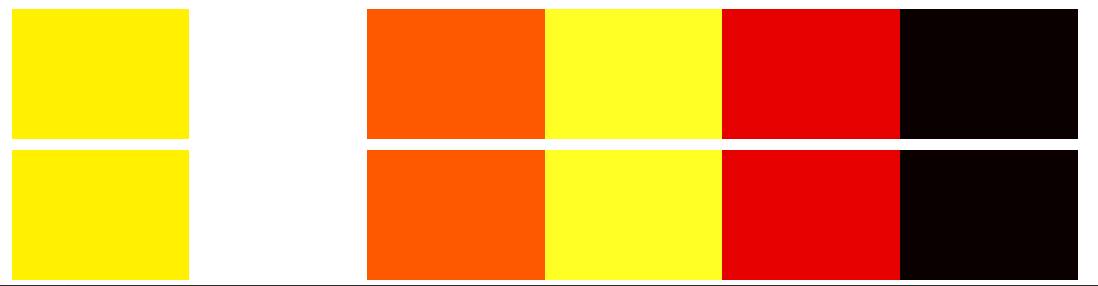
\includegraphics[scale=0.25]{timestamps.png}
    \centering
    \caption{\textit{Start} and \textit{End Timestamps} of PEs for a $1 \times 6$ \texttt{Resource Rectangle}}
    \label{fig:timestamps}
\end{figure}

\begin{table}[h]
    \centering
    \begin{tabular}{|c|c|}
        \hline
        Start Time & End Time \\
        \hline
        215471598885009 & 215471606612597 \\
        210033113389942 & 210033121118543 \\
        219951141230794 & 219951157273972 \\
        214324783517930 & 214324792236640 \\
        223219653123097 & 223219661842174 \\
        229732080439964 & 229732083089828 \\
        \hline
    \end{tabular}
    \caption{Device Timestamps used in the Heatmap in Figure \ref{fig:timestamps}}
    \label{table:timestamps}
\end{table}

Figure \ref{fig:timestamps} is a heatmap representing the start and end timestamps on the fabric created from data in table \ref{table:timestamps}, the lighter colors represent PEs that start first, the darker colors represent the PEs that started at a later point in time. Given the variation in timestamps across PEs which could depend on the hardware implementation of calls to the device. Our measurements calculate the min, mean and max differences between the start and end timestamps and uses the best measurement for the experiment since the tiling of the \textit{Distance Matrix} leads to tiles of various sizes which impacts the execution time.

\subsection{Low-Level (Kernel) Model} \label{subsection:low_level_model}

The algorithm to compute the Matrix profile as defined in Algorithm \ref{alg:tiled_matrix}, is an \(O(t_{s}^2)\) algorithm and computes the upper triangle of a given tile also called the half tile. The execution time is directly proportional to $t_s$. Our experiment look at the hardware and simulator runtimes on executions on a single PE solving a problem of size $s$ = $t_s$. Figure \ref{fig:execution_tiles_comparison} is a plot of execution times vs increasing tile sizes. We hence arrived at a Theoretical model for estimating runtime for a given tile size.

\begin{equation}
    T(t_s) = 4.38e^{-5} * t_s^2 + 1
    \label{eq:half_tile_execution}
\end{equation}

\subsection{Complete Tile Model} \label{subsection:complete_tile_model}

The complete tiles experiments were conducted by executing a complete tile in a single PE where $s$ > $t_s$. The results from the hardware and simulator are depicted in Figure \ref{fig:execution_tiles_comparison}. Thus, we arive at the theoretical model for the runtime of a complete tile. 

\begin{equation}
    T(t_s) = 1.001e^{-4} * t_s^2
    \label{eq:full_tile_execution}
\end{equation}

\begin{figure}[h!]
    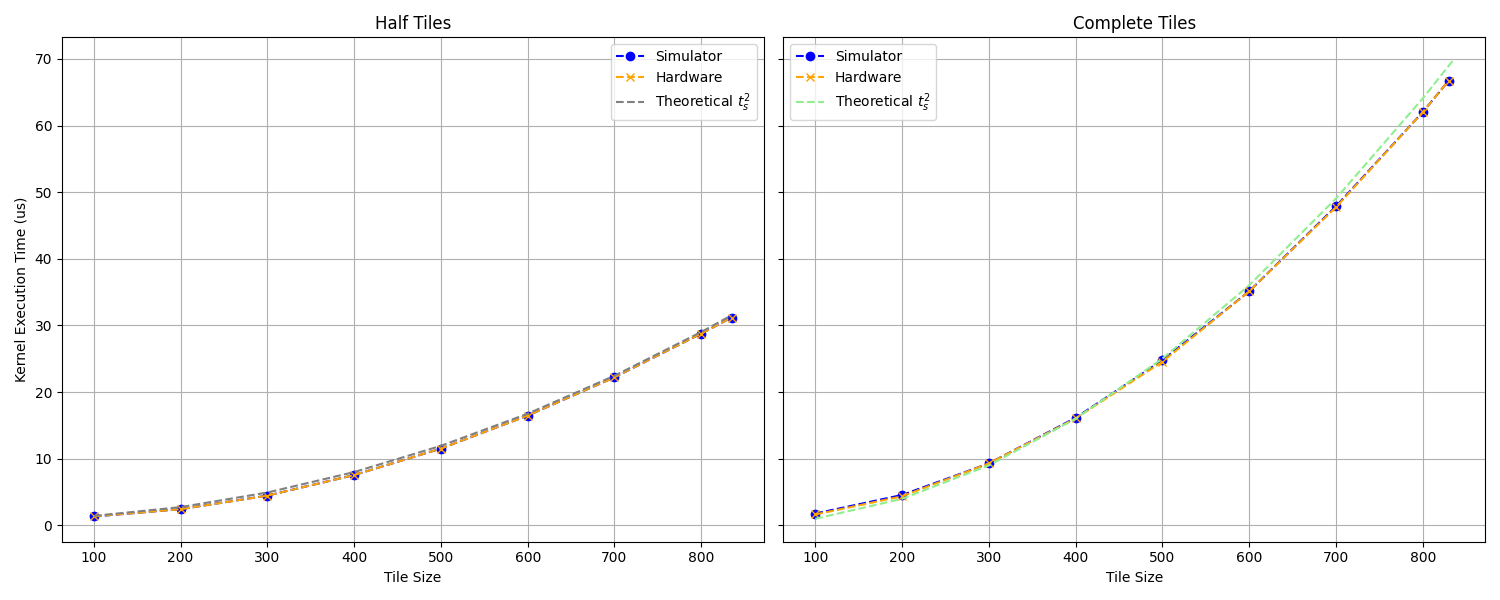
\includegraphics[scale=0.35]{execution_tiles_comparison.png}
    \centering
    \caption{Comparison of \textit{Kernel Execution Time} of increasing tile sizes $t_s$ on a single PE computing a half and complete tile.}
    \label{fig:execution_tiles_comparison}
\end{figure}

\section{Memory Consumption Model} \label{section:memory_consumption}

Matrix profiling is an memory intensive algorithm since it involves multiple variables and coefficients of data for computation, the Cerebras SDK does not expose any metrics on memory consumption. Hence, we present our mathematical model on memory usage on a single PE and compare it to what was practically possible to consume on the PE. The memory consumption $M$ for a single Processing Element (PE) in a Matrix Profiling computation of two time series $a$ and $b$ can be modeled using the following equation:


\[
M = F(inputs_a, inputs_b, outputs_a, outputs_b)
\]
\[ 
M = F(T_a, inf_a, df_a, dg_a, T_b, inf_b, df_b, dg_b, args, MP_a, MPI_a, MP_b, MPI_b)
\]

Upon further reduction, the equation becomes:

\[
M = \text{sizeof}(2 \times (t_s + m) + 10 \times (t_s - m + 1) + 7)
\]

Substituting the values for $t_s$ (tile size), $m$ (window size), size of each variable being 32 bits and simplifying, we get:

\begin{equation} \label{eq:memory_usage}
M = \frac{3 \times t_s - 2 \times m + 17}{256}
\end{equation}

Here, $t_s$ represents the tile size and $m$ represents the window size.

The plots demonstrate the relationship between memory consumption ($M$) and tile size ($t_s$). We set the window size $m$ to 6. Additionally, They include theoretical and practical limits for memory consumption. Figure \ref{fig:mem_usage} shows a plotted model using the Equation \ref{eq:memory_usage}. We reaching a practical limit of 39.01 KB on a maximum tile size $t_s$ of 835. We are able to allocate 81\% of memory available in the PE. This does not account for the allocations required by the PE for execution since the global memory is also used for the program instructions and other runtime allocations. For the following experiments, we set $t_s$ to 830 since we encountered higher errors when $t_s$ = 835 which we could not explain.

\begin{figure}[h!]
    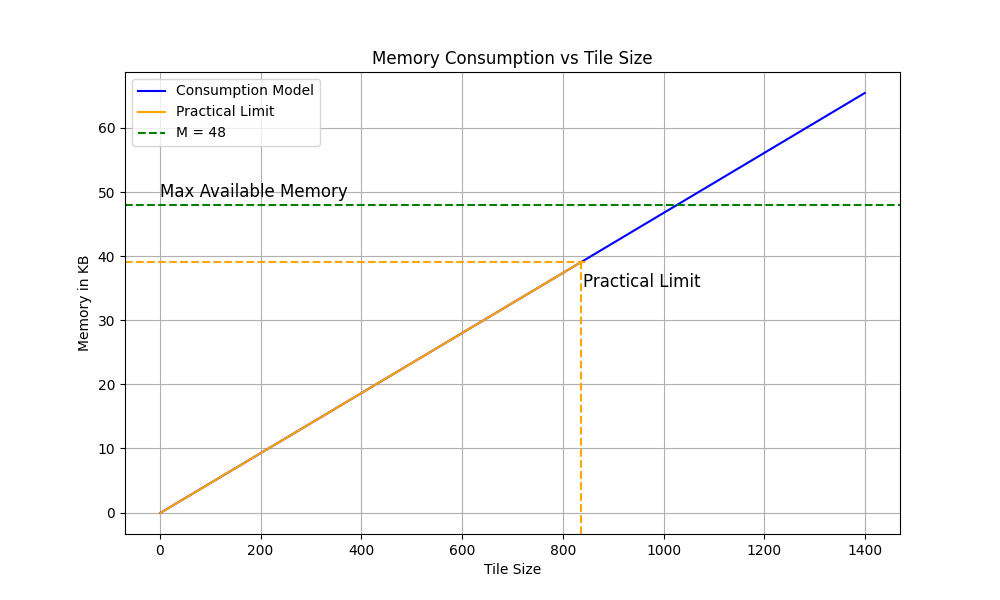
\includegraphics[scale=0.50]{memory_6}
    \centering
    \caption{Memory Usage (\textit{M}) of a single PE plotted against Tile Size $t_s$. The theoretical limit to $t_s$ is 1010 but what is observed is a maximum limit of 835 per PE. In practice, we were able to use 39.01 KB of memory of the 48KB available in a PE.}
    \label{fig:mem_usage}
\end{figure}


\section{Memory Bandwidth Experiments} \label{section:memory_bandwidth_experiments}

The following section contains experiments that try to evaluate the memory bandwidth of the Cerebras WSE-2 by executing Matrix Profiles of time series of increasing sizes. This enables us to model the memory latency and transfer times of the Cerebras WSE-2.

\subsection{Memory Bandwidth} \label{subsection:memory_bandwidth}

Our first experiment looks at the memory bandwidth capabilities of the Cerebras WSE-2 and the impact of the size $s$ of the time series. We fixed the tile size $t_s$ to 830 and gradually increased the time series size $s$ to transfer increasing quantity of data to the device. With a tile size of $t_s$ = 830, Each PE in this experiment receives 39.01 KB, and the total transfers range from 622 to 15562.37 KB to the device and 207.4 to 5187.4 KB from the device. This enables us to look at concrete differences in transfer times of large time series.

\begin{figure}[h!]
    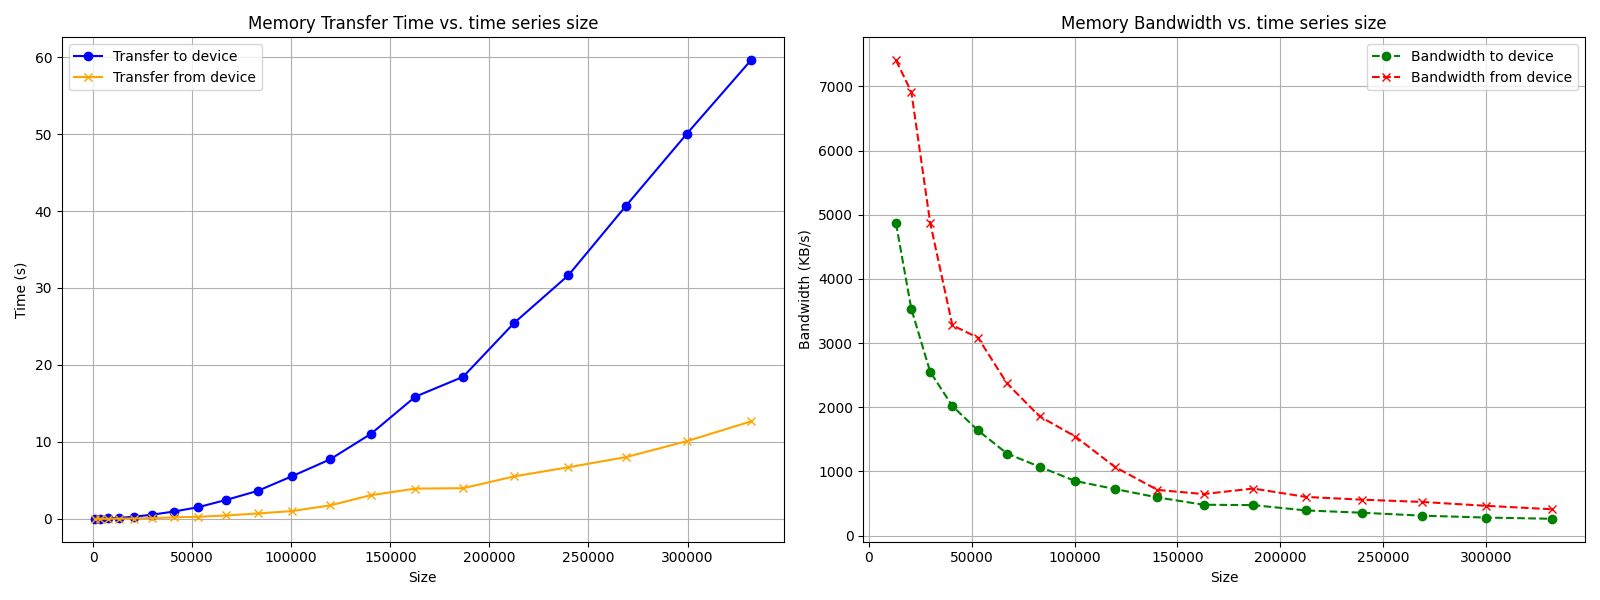
\includegraphics[scale=0.35]{memory_transfer_times_and_bandwidth_subplot.png}
    \centering
    \caption{\textit{Memory Transfer Time} in seconds and \textit{Bandwidth} in KB/s of time series of increasing sizes.}
    \label{fig:memory_bandwidth}
\end{figure}

In Figure \ref{fig:memory_bandwidth}, we notice a sharp decline in memory bandwidth of 27\% and this can be explained by the exponential increase in number of PEs allocated and the complexity of the \texttt{Resource Rectangle}. The WSE-2 contains 66 memory channels spaced evenly at almost 16 intervals at the two edges of the wafer. This allows data to be streamed into the PEs through multiple channels across the wafer\footnote{https://sdk.cerebras.net/tensor-streaming}. This experiment allocates large \texttt{Resource Rectangle} configurations of sizes $(70\times949)$, $(101\times806)$, etc. which uses almost the available memory channels on the wafer which could be a reason behind the decline in memory bandwidth.

We can then consider the memory transfer times $M_{t}$ and $M_{f}$ for a given time series of size $s$. We arrived at the following equations for transfer times to and from the device. This does not take into consideration the \texttt{Resource Rectangle} configurations since it also impacts the memory transfer times but as seen in Subsection \ref{subsection:wafer_location}, the impact is negligible.

\begin{equation}
    M_{t}(s) = 5.354e^{-10} \times s^2 + 4.843e^{-06} \times s + -1.207e^{-01}
    \label{eq:memory_to_device}
\end{equation}

\begin{equation}
    M_{f}(s) = 1.007e^{-10} \times s^2 + 4.400e^{-06} \times s + -1.014e^{-01}
    \label{eq:memory_from_device}
\end{equation}

\subsection{Impact of spacial location of PEs on the Wafer} \label{subsection:wafer_location}

We further explored the implication of different \texttt{Resource Rectangle} on the latency of data transfer to and from the device. This is essential since, the Cerebras WSE-2 does not have a classic hierarchial memory structure with multiple layers of cache. Each PE has access only to its global memory of 48KB and the data is transmitted through a network connection to the fabric. We choose to execute different tile sizes on different configurations of \texttt{Resource Rectangle} to observe the affect on memory transfer times. We represent the \texttt{Resource Rectangle} configurations using the two dimensions $w$ (Width) and $h$ (Height) to study the impact on latency of data transfer. The experiment was conducted on the device since the simulator does not provide accurate data transfer results. 

To study the impact of \texttt{Resource Rectangle} configurations on memory transfer, Our experiment consisted of $s$ = 10000, $t_s$ = 500, 600, 700 and $m$ = 6 and various $r\_r$ configurations. These sizes allow us to evaulate transfer rates of large volumes of data to and from the device and also create large enough resource rectangles that have a noticable impact on the memory transfer times. We fixed the width to 1 and expanded along the height, e.g. $1\times66, 1\times105, 1\times410$ and fixed the height to 1 and expanded along the width, e.g. $66\times1, 105\times1, 410\times1$ to deleve into the impact of different dimensions of the \texttt{Resource Rectangle}. As seen in Figure \ref{fig:rectangle}, the data to the device enters the fabric from the left end of the Wafer and exits from the right end. This has an influence on the memory transfer times to and from the PEs in the \texttt{Resource Rectangle} configurdation. This experiment transmits 468.62 KB of data to the fabric from the west edge.

\begin{figure}[h!]
    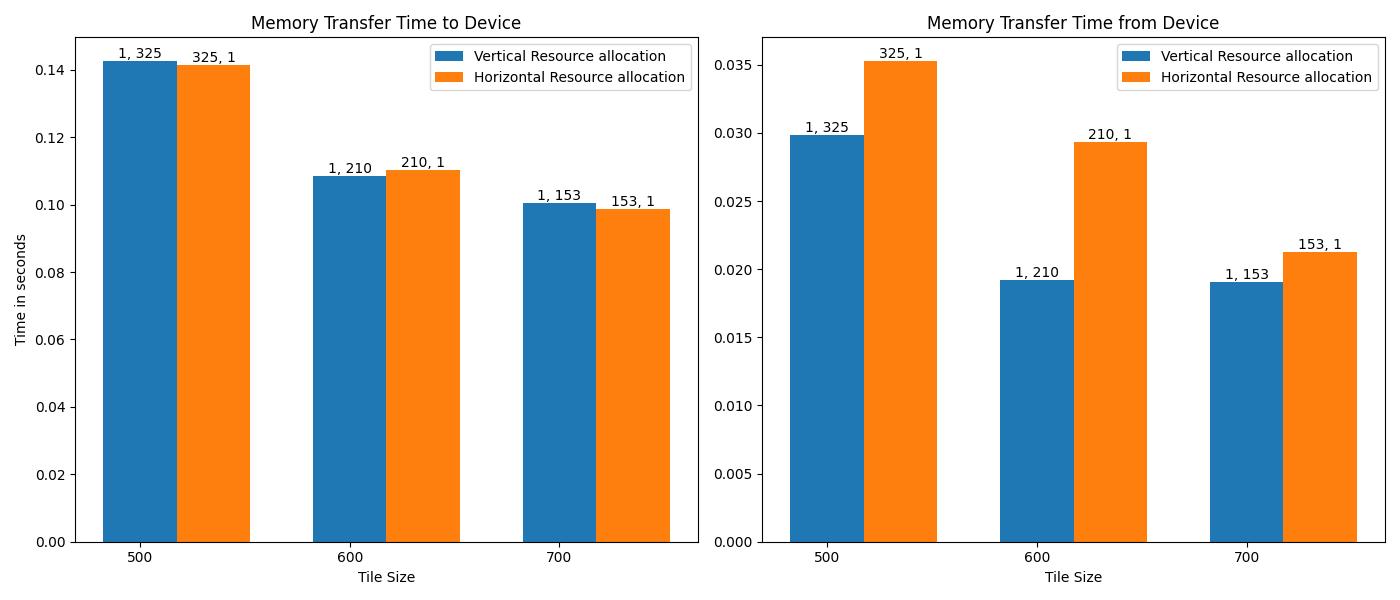
\includegraphics[scale=0.4]{memory_transfer_times_different_pe_config_1.png}
    \centering
    \caption{\textit{Memory Transfer time} on different resource rectangle configurations allocated at an offset of 4, 4 on the wafer.}
    \label{fig:memory_transfer_times_start}
\end{figure}

\begin{figure}[h!]
    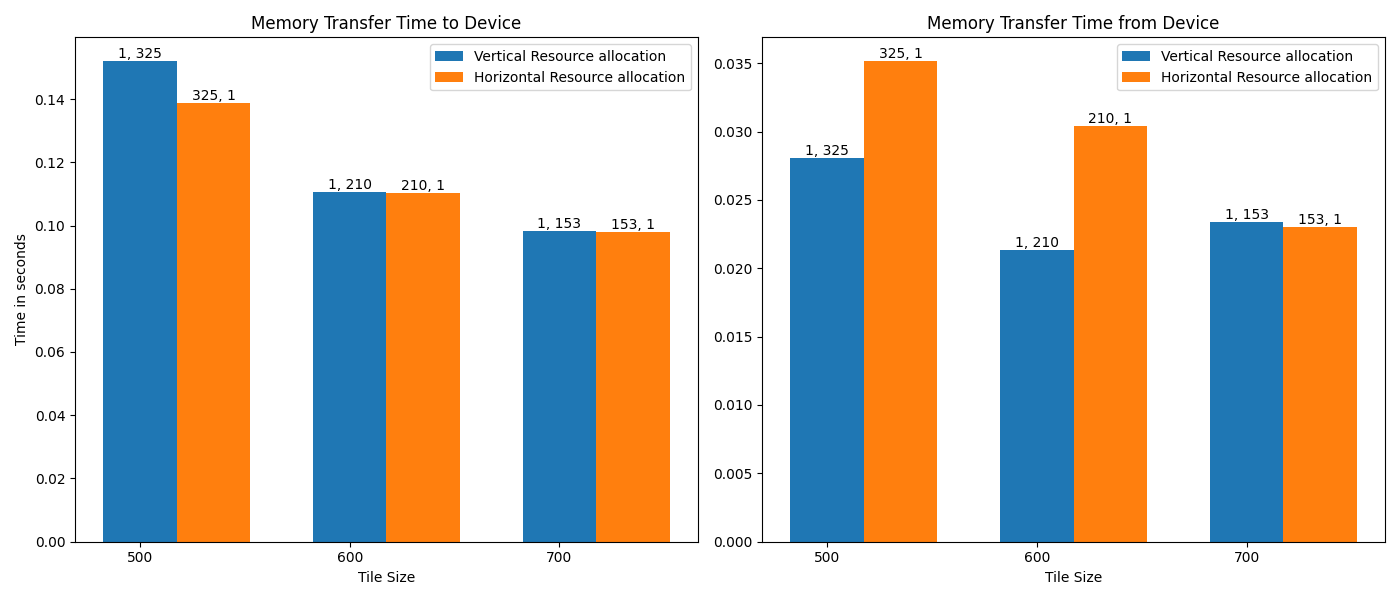
\includegraphics[scale=0.4]{memory_transfer_times_different_pe_config_2.png}
    \centering
    \caption{\textit{Memory Transfer time} on different resource rectangle configurations allocated at an offset of 300, 300 on the wafer.}
    \label{fig:memory_transfer_times_middle}
\end{figure}

Figure \ref{fig:memory_transfer_times_start} represents the transfer time to and from the device for a \texttt{r\_r} allocated at an offset of 4, 4 on the wafer. The above results are from $r\_r$ allocations at the top right corner of the fabric. This leads to almost equal transfer times to the device in different allocation patterns. The transfer times from the device show a pattern of greater (4\%) transfer times for horizontal resource allocations. This could be due to the overhead of data travelling through the same fabric since the PEs are allocated in the same row.

Figure \ref{fig:memory_transfer_times_middle} represents the transfer time to and from the device for a \texttt{r\_r} allocated at an offset of 300, 300 the wafer. We see a trend of higher transfer times for all shapes even though the variation is about 5\%. There is also a increase in transfer time from the device for horizontal resource allocations. The above figures show very slight variations (5\%) in transfer times and does not show any concrete impact of different \texttt{Resource Rectangle} configurations since we are dealing with millisecond differences.

\section{Time Series Execution Model} \label{subsection:time_series_model}

Now that we have a theoretical model for execution times for half and complete tiles for a given $t_s$ and memory transfer times for time series of a given size $s$, we can derive a model to predict the runtime of any given time series of size $s$, tiled into tiles of size $t_s$. Figure \ref{fig:total_execution_time} plots the total execution times of time series of increasing sizes. We notice a lower execution and memory transfer times on smaller time series and a gradual increase in memory transfer times to the device due to the increase in time series sizes and \texttt{Resource Rectangle} complexity.

\begin{figure}[h!]
    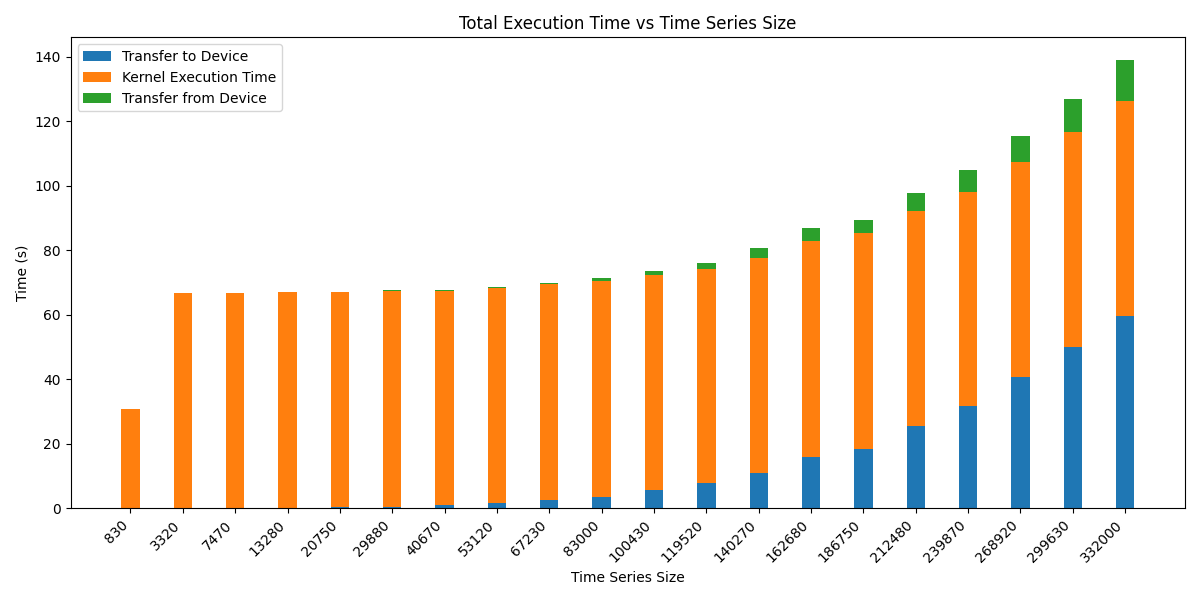
\includegraphics[scale=0.45]{total_execution_time.png}
    \centering
    \caption{\textit{Total Execution Times} for series of increasing sizes.}
    \label{fig:total_execution_time}
\end{figure}

From Figure \ref{fig:total_execution_time}, we can derive that when $t_s$ > $s / 2$, we notice a higher performance, this can be explained by the tiling nature and the presence of more half tiles in the computation. With this information, We arrive at the below formulation for the kernel execution time of a series of size $s$ and tile size $t_s$ in seconds, considering Equation \ref{eq:full_tile_execution} and \ref{eq:half_tile_execution}.

\begin{equation}
    T_{kernel}(s, t_s)= 
    \begin{cases}
        4.38e^{-5} * t_s^2 + 1,& \text{if } t_s > s \times 0.7\\
        1.001e^{-4} \times t_s^2,& \text{if } t_s \leq s / 2 
    \end{cases}
    \label{eq:kernel_execution}
\end{equation}

We can simplify this for normal time series of larger sizes and arrive at a final equation.

\begin{equation}
    T_{kernel}(t_s)= 1.001e^{-4} \times t_s^2
\end{equation}

Thus combining Equation \ref{eq:memory_to_device}, \ref{eq:memory_from_device} and \ref{eq:kernel_execution}, we arrive at a model for the total execution time ($T_{total}$) for any given time series of size $s$ and tile size $t_s$.

\[ T_{total}(s, t_s) =  M_t(s) + T(t_s) + M_f(s) \]

Substituting the equations for \( M_{to\_device}(s) \), \( T_{kernel}(s, t_s) \), and \( M_{from\_device}(s) \), we get

\[
    \begin{aligned}
        T_{\text{total}} &= M_t(s) + T(s, t_s) + M_f(s)
    \end{aligned}
\]

Substituting Equation \ref{eq:memory_to_device} and \ref{eq:memory_from_device}, we arrive at Equation \ref{eq:execution_model}

\begin{equation}
    \begin{aligned}
        T_{\text{total}} &= M_t(s) + T(s, t_s) + M_f(s) \\
        &= (\underbrace{5.354e^{-10} \times s^2 + 4.843e^{-06} \times s + -1.207e^{-01}}_{\text{Memory Transfer Time}} \\
        &\quad + \underbrace{1.001e^{-4} \times t_s^2}_{\text{Time for Compute}} \\
        &\quad + \underbrace{1.007e^{-10} \times s^2 + 4.400e^{-06} \times s + -1.014e^{-01}}_{\text{Memory Fetch Time}})
    \end{aligned}
    \label{eq:execution_model}
\end{equation}

This is the model to find out the execution time of a time series of any given size on the Cerebras WSE-2. Note that this does not take into account the resource availability on the wafer or the presence of clusters containing multiple such wafers.

\begin{figure}[h!]
    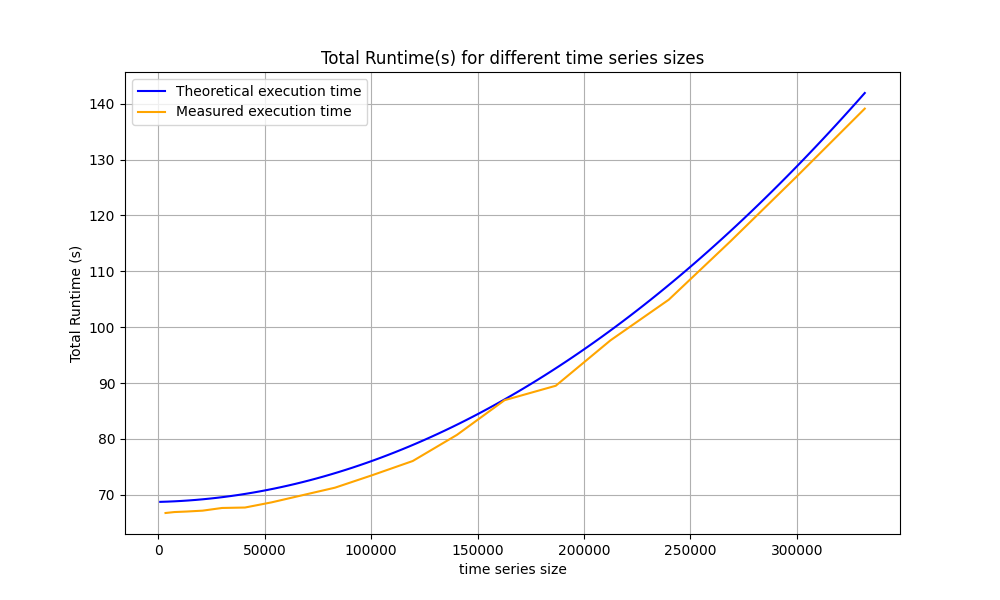
\includegraphics[scale=0.50]{theoretical_execution_model.png}
    \centering
    \caption{\textit{Total Execution Time}: Aggregate execution times comprising both memory transfer and kernel execution times for time series of increasing sizes.}
    \label{fig:theoretical_execution_model}
\end{figure}

Figure \ref{fig:theoretical_execution_model} presents the theoretical execution model vs total execution times of time series of increasing sizes. We see variations in the execution times which could be explained by the influence of different \texttt{Resource Rectangle} configurations on the transfer times.

\section{Weak Scaling Experiment} \label{section:weak_scaling}

Since the WSE-2 primarily focuses on weak scaling, we examine the potential implications of weak scaling on the device using various configurations and analyze the execution times. We initiate our weak scaling experiments by gradually increasing the number of resources allocated for the time series. We use the following equation: \[ s = i^2 \times t_s \] Where \( t_s \) = 830 and \( i \) ranges from 1 to 20. This provides us with an exponential increase in the sizes of the \texttt{Resource Rectangle} and a constant execution time for all PEs since \( T_{kernel}(s) \propto t_s \).

The execution times represent the maximum execution time of all the PEs in the \texttt{Resource Rectangle} since there can be multiple PEs with lower workloads given the smaller tile dimensions. Weak scaling is evident when comparing the performance metrics across different problem sizes. Despite the increase in problem size, the performance metrics remains the same with increasing computational resources, maintaining a consistent workload per processing element.

\begin{figure}[h!]
    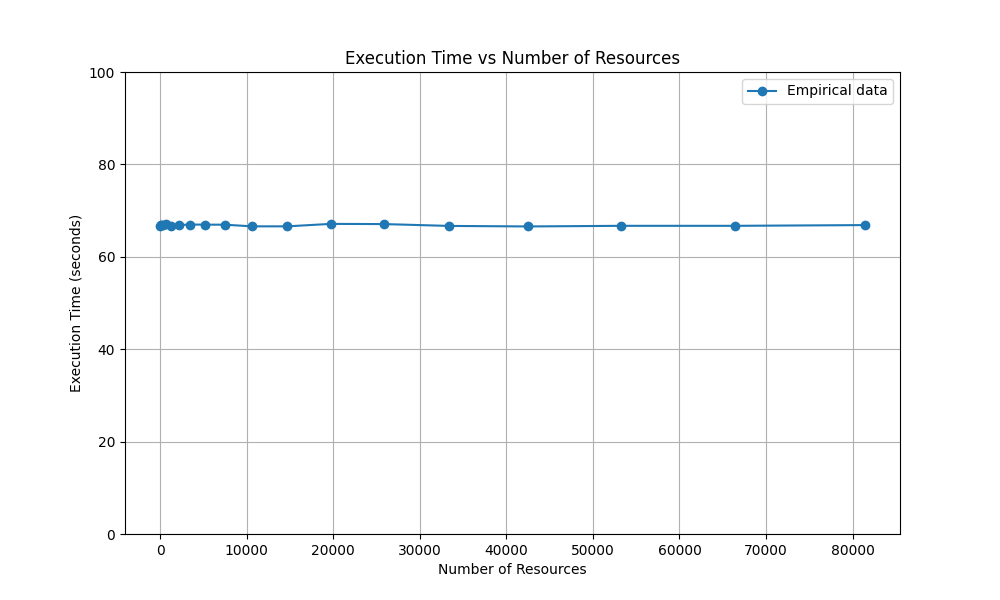
\includegraphics[scale=0.5]{weak_scaling.png}
    \centering
    \caption{\textit{Weak Scaling} effects of the Cerebras WSE-2 on large time series.}
    \label{fig:weak_scaling}
\end{figure}

\section{Strong Scaling Experiment} \label{section:strong_scaling}

Although the Cerebras WSE-2 is not built with strong scaling in mind, we planned our strong scaling experiments in the following manner, We tested the \textit{Tiled Kernel} with different number of PEs while keeping the problem size constant. We keep $s$ = $10000$ and decreasing $t_s$. $t_s$ is continuously decreased from $830$ to $100$ which also leads to a increase in the amount of resource required for computation. In theory, We expect a decrease in the computation time given the increase in resources. The results of the experiment are depicted in Figure \ref{fig:strong} with the execution time on logscale.

\begin{figure}[h!]
    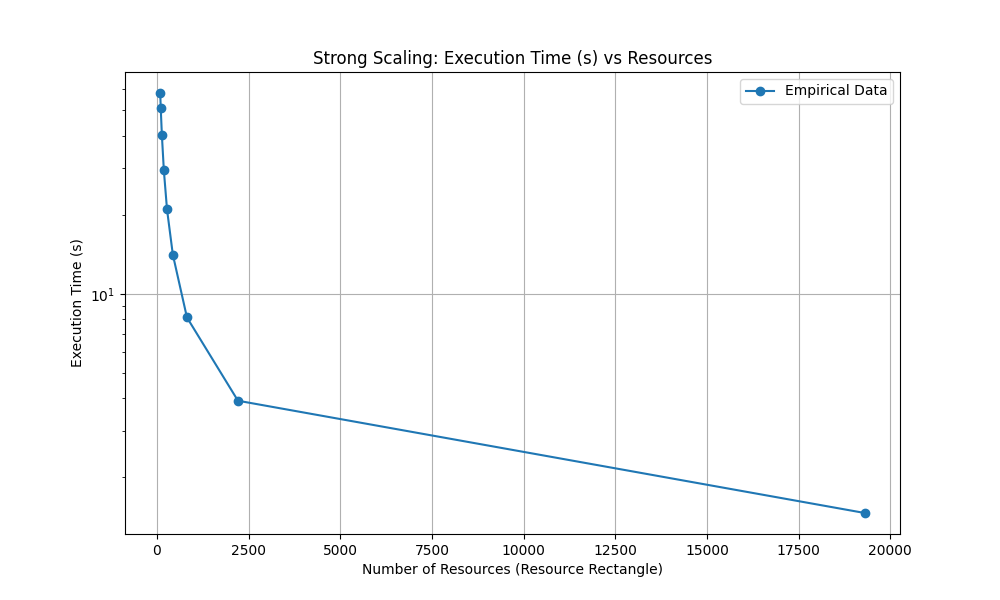
\includegraphics[scale=0.5]{strong_scaling}
    \centering
    \caption{\textit{Strong Scaling} - Kernel Execution time with increasing \texttt{Resource Rectangle} sizes}
    \label{fig:strong}
\end{figure}

We notice a lower execution times on the smaller time series due to the decompositional behaviour of the \textit{Distance Matrix}. Lower sizes of time series decompose into more half tiles which leads to lower mean execution times on the device. On the other hand, larger time series have more complete tiles which take around 66 seconds to compute, hence resulting in a almost straight line.

\section{Precision Evaluation} \label{section:precision_eval}

Given the unpredictable nature of real-world data, which often includes numerous constant areas, numerical instability arises as a concern. The similarity of z-normalized subsequences is of particular interest to many researchers. In constant regions, the standard deviation is zero. Additionally, near-constant subsequences pose challenges as they may pass a bit-level test for two distinct values, yet result in division by a number nearly approaching zero.

In this section, we take a look at the impact of Cerebras lower precision floating point limitation. In the experiment, we created and executed time series using different random distributions of size $s$ = 10000 and $m$ = 400 on the device. These results are then compared to the double precision version of SCAMP. Although this does not reflect on the error rates of real life dataset, we wanted to look at anomalies in error rates across different distributions. 

\begin{figure}[h!]
    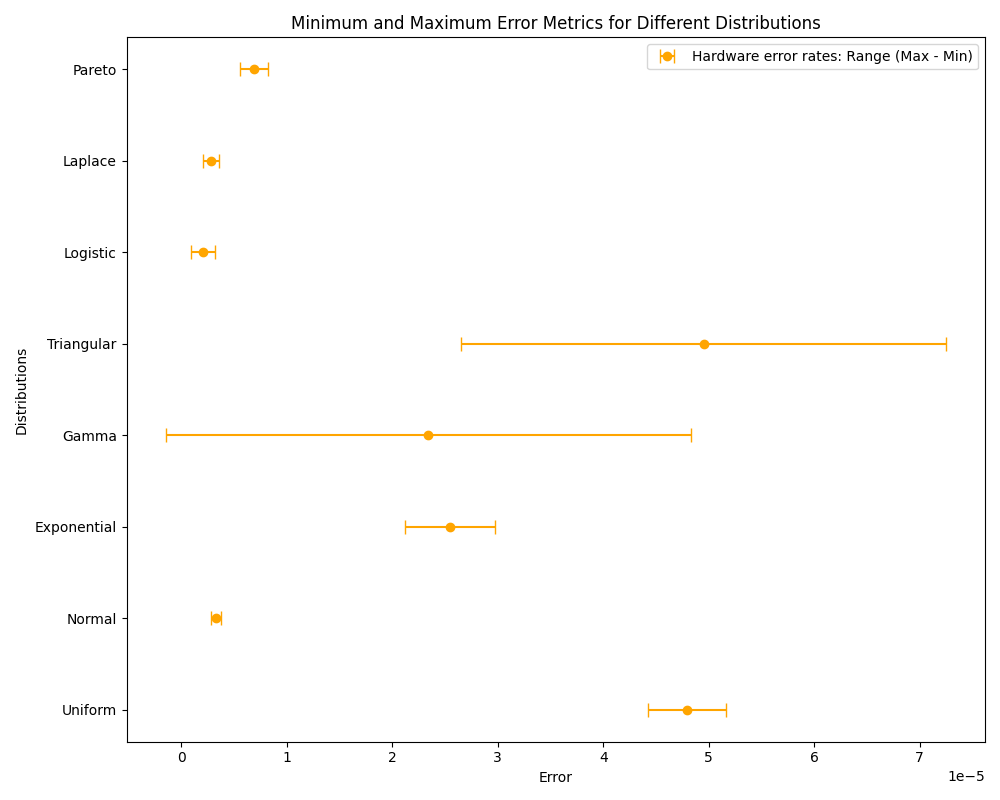
\includegraphics[scale=0.45]{error_distributions}
    \centering
    \caption{Error rate on different probabilistic distributions}
    \label{fig:error_distribution}
\end{figure}

The errors observed in Figure \ref{fig:error_distribution} on different error distributions reveal varying challenges and successes in accurately capturing the characteristics of each distribution. These error rates are crucial in assessing the accuracy and reliability of the Matrixc Profile. For instance, when considering the Uniform distribution, which exhibits a constant probability density function within a defined range, the error rates are relatively low across the board. This indicates that the Matrix Profile closely align with the actual values for this distribution, likely because the uniform nature of the data allows for more straightforward motif discovery.

On the other hand, distributions such as Triangular, Gamma, and Exponential, which possess more complex shapes and variability in their probability density functions, exhibit higher error rates. This suggests that the algorithm may struggle to accurately capture the nuances and variability present in these distributions, leading to larger discrepancies between predicted and actual values.

\clearpage

\section{Comparison to CPU \& GPU Baseline} \label{section:comparison_to_cpu_gpu}
 
Now that experimental results from both the simulator and hardware are available, along with a theoretical model for estimating total execution time for any given time series size $s$ and tile size $t_s$, a performance comparison between the Cerebras WSE-2 and traditional GPUs can be conducted. Table \ref{tbl:performance} presents an analysis of SCAMP performance on random walk datasets of increasing lengths \cite{4}, alongside extrapolated figures for the Cerebras WSE-2. 

Notably, due to limitations in the number of tiles executable in a single iteration and the cost of memory transfers to and from the device, significant disparities in execution times are observed.

\begin{table}[h!]
    \centering
    \renewcommand{\arraystretch}{1.25} % Adjust the spacing between rows
    \caption{Matrix Profiling Runtime on SCAMP on GPUs and our implementation on the Cerebras WSE-2 \cite{4}}
    \begin{tabular}{|| c | c | c | c ||} 
        \hline
        Implementation & \multicolumn{2}{c|}{SCAMP-GPU} & Cerebras \\ [0.5ex] 
        \hline
        Architecture & V100 & V100 & WSE-2 \\
        \hline
        Precision & DP & SP & SP \\
        \hline\hline
        $2^{18}$ & 3.04s & 0.34s \textbf{(8.9x)} & 1.9m \textbf{(3650.00x)} \\
        \hline
        $2^{19}$ & 11.4s & 1.24s \textbf{(9.2x)} & 4.14m \textbf{(2078.95x)}\\
        \hline
        $2^{20}$ & 44.1s & 4.81s \textbf{(9.2x)} & 12.96m \textbf{(1663.27x)} \\
        \hline
        $2^{21}$ & 174s & 19.0s \textbf{(9.2x)} & 48.09m \textbf{(1557.24x)} \\
        \hline
        $2^{22}$ & 629s & 69.2s \textbf{(9.1x)} & 188.29m \textbf{(1696.09x)} \\
        \hline
        $2^{23}$ & 2514s & 277s \textbf{(9.1x)} & 748.46m \textbf{(1686.30x)} \\
        \hline
    \end{tabular}
    \label{tbl:performance}
\end{table}

The execution times on the Cerebras WSE-2 are exponentially larger compared to SCAMP-GPU implementations. This is primarily due to the inherent latency introduced by memory transfers to and from the wafer, which significantly impacts the overall execution time. 

It's worth noting that for time series larger than $2^{22}$, the execution times become extremely long, with a time series of size 8M taking approximately 9 hours to execute without considering the overhead of the SLURM scheduler when running them on the EPIF. Hence, the derived execution times for larger datasets on the Cerebras WSE-2 are based on the theoretical model presented in Section \ref{subsection:time_series_model}.

\clearpage

\section{Execution on Real World Datasets} \label{section:real_world_datasets}

The real world dataset used in our evaluation of the Cerebras WSE-2 is StarLightCurves\footnote{https://www.cs.ucr.edu/\%7Eeamonn/time\_series\_data\_2018/}, consisting of a time series depicting the brightness of a celestial object over time. The examination of light curves in astronomy is integral to understanding source variability. Comprising 1 million entries, this dataset is sourced from the UCR Time Series Classification Archive \cite{UCRArchive2018}. Its distance matrix decomposes into 2,692,360 tiles, where $t_s = 830$ and $m = 400$. As this surpasses the 745,500 user-programmable PEs available on a single wafer, we segmented the problem and executed the dataset iteratively using our approach as described in Section \ref{section:iterative}.

We were unable to allocate the entire wafer for computation due to bandwidth limitations on Remote Procedure Calls (RPC) to the device for data transfers exceeding 2GB. Consequently, we allocated a maximum \texttt{Resource Rectangle} of $457 \times 696$ on the device, necessitating 8 iterations to compute the entire matrix profile. This limitation stems from the restricted memory availability of the PEs. With a maximum $t_s = 830$, larger time series require further segmentation, exacerbating overall time consumption due to average roundtrip execution time. An average execution time of $45s$ per PE was observed, lower than that for a tile size of $t_s = 830$, yet the rationale behind this discrepancy remains elusive. Figure \ref{fig:real_world_execution} illustrates the total execution time for each iteration.

\begin{figure}[h!]
    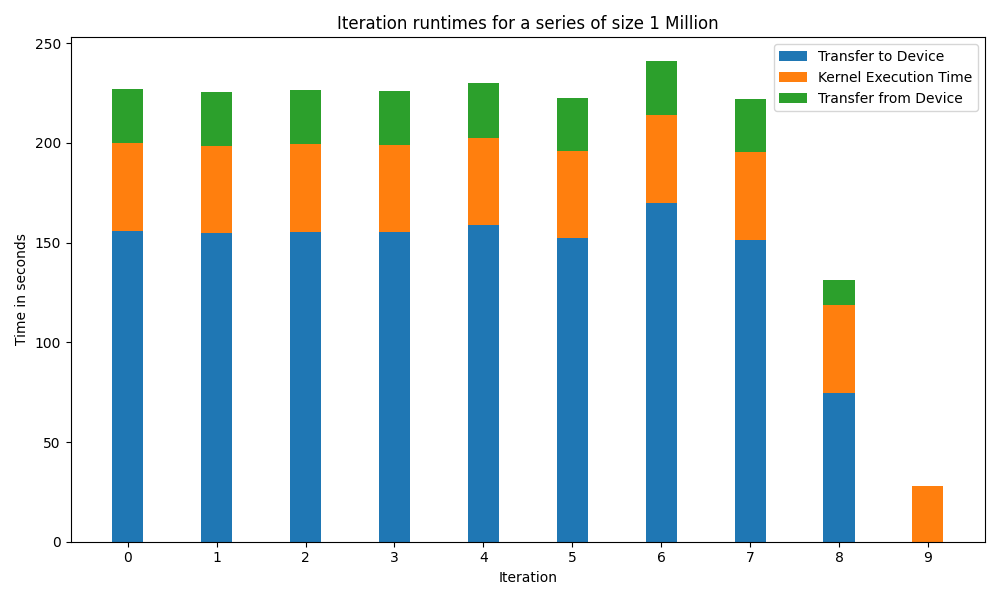
\includegraphics[scale=0.45]{real_world_execution.png}
    \centering
    \caption{\textit{Total Execution Time} of different iterations on a time series of size 1M}
    \label{fig:real_world_execution}
\end{figure}

We notice varying memory transfer times for the same allocated \texttt{Resource Rectangle} but see a similar execution time over all iterations. We achieved a absolute mean error rate of $1.865 \times 10^{-04}$ when compared to the double precision profile computed by SCAMP. Table \ref{tbl:max_absolute_error} compares the maximum absolute error of the Pearson Correlation for large datasets on SCAMP with Cerebras WSE-2. We were able to obtain comparable errors on the device.

\begin{table}[h!]
    \centering
    \renewcommand{\arraystretch}{1.25} % Adjust the spacing between rows
    \caption{Maximum absolute error (Pearson Correlation) for
    various datasets/algorithms, compared to SCAMP double precision results, taken from \cite{4}. StarLightCurves results were performed on the Cerebras WSE-2}
    \begin{tabular}{|| c | c | c | c ||} 
        \hline
        Size (m) & SCAMP SP & STOMP SP & Cerebras WSE-2 \\ [0.5ex] 
        \hline\hline
        Whitefly EPG (2.5M) & $3.75 \times 10^{-2}$ & $1.89 \times 10^{1}$ & N/A \\
        \hline
        ECG (8.4M) & $3.14 \times 10^{-4}$ & $2.07 \times 10^{-3}$ & N/A \\
        \hline
        Earthquake (1.7M) & $6.35 \times 10^{-1}$ & $3.17 \times 10^{3}$ & N/A \\
        \hline
        Power Demand (10M) & $4.85 \times 10^{-2}$ & $2.22 \times 10^{-1}$ & N/A \\
        \hline
        Chicken (9M) & $4.92 \times 10^{-2}$ & $2.27 \times 10^{1}$ & N/A \\
        \hline
        \textbf{StarLightCurves (1M)} & \textbf{$3.34 \times 10^{-4}$} & \textbf{$2.17 \times 10^{-2}$} &  \textbf{$1.865 \times 10^{-4}$} \\
        \hline
    \end{tabular}
    \label{tbl:max_absolute_error}
\end{table}

The Cerebras WSE-2 performs well on the StarLightCurves dataset since the values were in the order of $10^{-10}$. This could be represented precisely by single precision floats.